\subsection{Visual representation}
\label{sec:seg_colors}
For visually representing segmentation, we make a color map over the images, following
the cityscapes color palette \cite{cordts_cityscapes}. See figure \ref{fig:segmentation_colors}
for the exact palette and class list, and figure \ref{fig:cs_sample} for an example.

\begin{figure}[ht]
	\begin{center}
	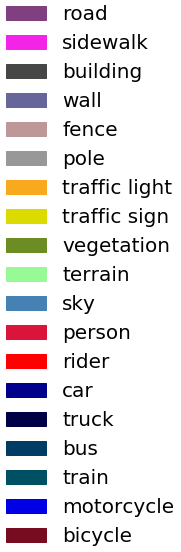
\includegraphics[width=0.2\textwidth]{./figures/seg_colors.png}
	\caption[Segmentation color palette]{
        Segmentation color palette.
        }
	\label{fig:segmentation_colors}
	\end{center}
\end{figure}

\begin{figure}[ht]
	\begin{center}
	\includegraphics[width=1\textwidth]{./figures/cityscapes_sample.png}
	\caption[CityScapes sample]{
        CityScapes sample.
        }
	\label{fig:cs_sample}
	\end{center}
\end{figure}

\subsection{Segmentation distribution}
\label{sec:seg_distribution}
Given the domain shift from Cityscapes to PlacePulse, is important to check how
the segmentation behaves on the new dataset.

The most significant difference between the datasets is the image size, which are almost 13
times bigger in cityscapes, allowing for smaller objects like traffic signs to be clearly
distinguishable. In training CS images are used with size of $769 \times 769$, while
place pulse images are used with the standard $224\times224$. Another important difference
is the origin of the images, while Cityscapes images were all taken on different cities of
the same developed country (Germany), PlacePulse images come from 56 cities distributed on all
continents, including both developed and developing countries, with the later ones contributing
images with a significant visual difference.

Table \ref{tab:segmentation} show the percentage of pixels belonging to each segmentation class
on the entire set of images of the PlacePulse dataset. Evidently this are not ground truth labels,
but the ones obtained by our  PspNet trained on Cityscapes. As was expected, classes representing
physically smaller objects have an almost negligible contribution since the smaller image size renders
them pretty much unidentifiable. Domain shift makes the model constantly confuse the sidewalk (which can
be seen in a large percentage of PlacePulse images) with the main road, reducing the class presence
to a very underwhelming 0.96\%. Same behavior can be perceived with the terrain class.


\begin{table}[H]
	\begin{tabular}{|l|r|} \hline
	Segmentation Class & \% of pixels \\ \hline
	Building      & 26.60\% \\
	Vegetation    & 25.52\% \\
	Road          & 24.21\% \\
	Sky           & 6.24\%  \\
	Fence         & 5.09\%  \\
	Truck         & 2.96\%  \\
	Car           & 1.94\%  \\
	Person        & 1.48\%  \\
	Bicycle       & 1.36\%  \\
	Motorcycle    & 1.28\%  \\
	Sidewalk      & 0.96\%  \\
	Wall          & 0.89\%  \\
	Terrain       & 0.65\%  \\
	Pole          & 0.33\%  \\
	Train         & 0.26\%  \\
	Bus           & 0.14\%  \\
	Traffic sign  & 0.05\%  \\
	Traffic light & 0.02\%  \\
	Rider         & 0.02\%  \\ \hline
	\end{tabular}
	\caption[Segmentation Distribution]{
		Pixel distribution of the segmentation classes over the PlacePulse Dataset
	}
	\label{tab:segmentation}
\end{table}